% =====================================================================
% a0z paper: "Epoch-Dependent Acceleration Scale from Bounded Topology:
%             Predictions for High-Redshift Galactic Dynamics"
% Author: B. Shatto
% Preprint, single-column article class, for open-archive deposit.
%
% Build:
%   pdflatex a0z-paper
%   pdflatex a0z-paper
% (Bibliography is inlined as thebibliography; no bibtex pass required.
%  references.bib is kept alongside for optional bibtex regeneration.)
% =====================================================================

\documentclass[11pt,a4paper]{article}

% --- core packages ---------------------------------------------------
\usepackage[utf8]{inputenc}
\usepackage[T1]{fontenc}
\usepackage{lmodern}
\usepackage{microtype}
\usepackage[a4paper,margin=1in]{geometry}
\usepackage{amsmath,amssymb}
\usepackage{mathtools}
\usepackage{graphicx}
\usepackage{booktabs}
\usepackage{array}
\usepackage{xcolor}
\usepackage[colorlinks=true,linkcolor=blue!50!black,citecolor=blue!50!black,
            urlcolor=blue!50!black]{hyperref}
\usepackage[numbers,sort&compress]{natbib}
\usepackage{enumitem}
\usepackage{caption}
\usepackage{authblk}

% --- numbering -------------------------------------------------------
\numberwithin{equation}{section}
\numberwithin{table}{section}
\numberwithin{figure}{section}

% --- spacing ---------------------------------------------------------
\setlength{\parskip}{0.4em}
\renewcommand{\arraystretch}{1.15}

% --- float placement: keep [!ht] floats tight to their prose ---------
\renewcommand{\topfraction}{0.9}
\renewcommand{\bottomfraction}{0.8}
\renewcommand{\textfraction}{0.07}
\renewcommand{\floatpagefraction}{0.7}
\setcounter{topnumber}{3}
\setcounter{bottomnumber}{2}
\setcounter{totalnumber}{4}

% --- figures path ----------------------------------------------------
\graphicspath{{../figures/}{./figures/}}

% --- shorthand macros ------------------------------------------------
\newcommand{\Mob}{\ifmmode\text{M\"obius}\else M\"obius\fi}
\newcommand{\afid}{a_0}
\newcommand{\Msun}{M_\odot}
\newcommand{\vflat}{v_\text{flat}}
\newcommand{\Mb}{M_b}
\newcommand{\Mdyn}{M_\text{dyn}}
\newcommand{\rM}{r_M}
\newcommand{\tff}{t_\text{ff}}
\newcommand{\geff}{g_\text{eff}}
\newcommand{\gN}{g_N}
\newcommand{\Hz}{H(z)}
\newcommand{\Ez}{E(z)}
\newcommand{\Cval}[1]{C(#1/120)}
\newcommand{\Mhalo}{M_\text{halo}}
\newcommand{\Rvir}{R_\text{vir}}
\newcommand{\rhocrit}{\rho_\text{crit}}
\newcommand{\NFW}{M_\text{NFW}}

% =====================================================================

\title{Epoch-Dependent Acceleration Scale from Bounded Topology:\\
       Predictions for High-Redshift Galactic Dynamics}

\author[1]{B.~Shatto\thanks{%
   Email: \href{mailto:bshatto.pe@gmail.com}{bshatto.pe@gmail.com}.\
   ORCID: \href{https://orcid.org/0009-0007-4419-1311}{0009-0007-4419-1311}.}}
\affil[1]{St.~Petersburg, FL, USA}

\date{\today}

\begin{document}

\maketitle

% =====================================================================
\begin{abstract}
We propose that the MOND acceleration scale evolves with cosmic epoch as
$\afid(z) = \afid(0)\,\Ez$, where $\Ez = \Hz/H_0$. This single input
predicts five correlated high-redshift observables: BTFR normalization
($E^{-1}$), MOND transition radius ($E^{-1/2}$), asymptotic velocity at
fixed baryonic mass ($E^{+1/4}$), Newtonian-inferred lensing mass
enhancement ($E^{+1/2}$), and collapse-time shortening ($E^{-1/4}$). The
prediction is calibrated to the local SPARC value and compared with the
KMOS3D Tully--Fisher offsets, where it faces a $2.9\sigma$ trend-shape
tension under conservative systematics. Its sharpest near-term test is
Euclid DR1 stacked galaxy--galaxy lensing at $z = 0.5$--$2$: the model
predicts a mass- and aperture-independent $74\%$ enhancement of
$\Mdyn/\Mb$ at $z = 2$, unlike the mass- and aperture-dependent
evolution expected from $\Lambda$CDM halo concentration. The topological
mechanism fixing $\afid/(cH) = 0.1845$ is presented in
Section~\ref{sec:derivation} and Appendix~\ref{app:framework}.
\end{abstract}

% =====================================================================
\section{Introduction}
\label{sec:intro}

The MOND acceleration scale $\afid \approx 1.20 \times 10^{-10}$~m/s$^2$
has governed the phenomenology of galactic rotation curves for four
decades \citep{Milgrom1983}. Fitted to the local SPARC sample with
intrinsic scatter of 0.1~dex \citep{Lelli2016,Famaey2012}, it satisfies
a numerical coincidence that has never been explained:
$\afid/(cH_0) \approx 0.18$, with the Hubble rate setting the
dimensional scale of the MOND threshold
\citep{Milgrom1999,McGaugh2004}. Within standard MOND this ratio is an
accident; within $\Lambda$CDM it has no physical correlate at all. It
has remained unexplained since Milgrom first noted it in 1983.

Two current problems motivate examining this scale across cosmic time.

First, the coincidence itself. Using the standard SPARC normalization
\citep{Lelli2016} and Planck 2018 $H_0$ \citep{Planck2018},
$\afid/(cH_0) = 0.183$, numerically stable across four decades of
improving measurements with no theoretical account of why.

Second, JWST has revealed candidate galaxies at $z \sim 7$--$10$ with
stellar masses $M_\star \gtrsim 10^{10}\,\Msun$ assembled within
600~Myr of the Big Bang \citep{Labbe2023,BoylanKolchin2023}. Under
standard halo-growth assumptions, the most extreme candidates imply
unusually high star-formation efficiencies and have been discussed as a
potential early-structure tension. If $\afid$ were larger at early
times, gravitational collapse would proceed faster and the tension
would ease. A related application to the DESI DR2 dark-energy signal
\citep{DESI2025} is treated in a separate preprint; this paper is
limited to the galactic-dynamics consequence of an epoch-dependent
$\afid$.

This paper develops one hypothesis and its consequences. Within a
bounded-topology measurement framework on
$S^1 = \partial(\Mob) \hookrightarrow S^3$
(Appendix~\ref{app:framework}), the Milgrom ratio resolves to the ratio
of two phase-operator values at Fibonacci wells on the 120-domain
native to $S^3/2I$:
\begin{equation}
\frac{\afid}{cH} = \frac{\Cval{13}}{\Cval{34}} = 0.1845,
\label{eq:milgrom-ratio}
\end{equation}
agreeing with the observed $0.1833$ at the $0.7\%$ level. The ratio
itself is not a separate adjustable parameter: once the $\afid$ and $H$
wells are fixed by separately calibrated well assignments sharing the
same edge-mode hierarchy, \eqref{eq:milgrom-ratio} follows
algebraically. The non-trivial content is the $0.7\%$ match at a
combinatorially sparse position (Section~\ref{sec:derivation}). Among
the framework's six Fibonacci-well pairs, $(13, 34)$ is the unique pair
that reproduces the observed ratio within $1\%$
(Section~\ref{sec:derivation}).

Because both $\afid$ and $H$ reference the same epoch-dependent
hierarchy in the framework's scaling law, the ratio
\eqref{eq:milgrom-ratio} holds at every cosmic epoch. The evolution
follows:
\begin{equation}
\afid(z) = \afid(0)\,\Ez, \qquad \Ez \equiv \Hz/H_0.
\label{eq:evolution}
\end{equation}

The bare possibility $\afid \propto H$ has appeared previously in
MOND-motivated discussions of the Milgrom coincidence. The novelty here
is not the dimensional guess, but the specific framework mechanism: the
ratio is fixed by $\Cval{13}/\Cval{34}$, the evolution is linear in
$\Ez$, and the five observable exponents are locked together rather
than tuned independently.

Five testable predictions follow as different powers of $\Ez$, with no
additional free parameter beyond the local SPARC calibration. The
Euclid DR1 release in October 2026 will deliver the sharpest test
through stacked galaxy--galaxy weak lensing at $z = 0.5$--$2$. The
framework's monotonic BTFR prediction is currently in tension with the
only existing intermediate-redshift measurement \citep{Ubler2017}; this
tension is quantified in Section~\ref{sec:constraints}.

Section~\ref{sec:derivation} derives \eqref{eq:milgrom-ratio} and
\eqref{eq:evolution}. Section~\ref{sec:channels} propagates the
evolution into five observable channels.
Section~\ref{sec:constraints} treats existing constraints.
Section~\ref{sec:euclid} specifies the Euclid test.
Section~\ref{sec:conclusions} closes.

% =====================================================================
\section{Derivation}
\label{sec:derivation}

The framework's measurement postulate (Appendix~\ref{app:framework})
maps any Planck-normalized observable to a phase position on the
120-domain native to $S^3/2I$:
\begin{equation}
\frac{A}{A_P} = C(\Theta) \cdot N^n,
\qquad C(\Theta) = 2\sin^2(\pi\Theta),
\label{eq:scaling-law}
\end{equation}
where $\Theta \in \{k/120\}$ is the phase position, $n$ the
manifold-mode index set by the embedding hierarchy
$S^1 \subset \Mob \subset S^3$, and $N$ a dimensionless hierarchy
normalization that takes the form $(\sqrt{\Omega})^{-1}$ within each
mode class, with its exact value fixed by calibrating one reference
observable per sector. The phase operator $C(\Theta)$ is the squared
ground-mode intensity on the \Mob{} surface under anti-periodic
boundary conditions (Appendix~\ref{app:120-domain}). A selection rule
assigns edge-mode observables ($n = 1$) to the kinematic hierarchy
$\Omega_H$ and surface-mode observables ($n = 2$) to the eigenvalue
hierarchy $\Omega_\Lambda$ (Appendix~\ref{app:selection}). The
normalization $N$ is associated with the embedding hierarchy: for edge
modes ($n = 1$), the relevant kinematic hierarchy is
$\Omega_H(z) = (c/(H(z)\ell_P))^2$, giving the leading scale
$N_H \sim H(z)\,t_P$, while the calibrated framework normalization used
below is fixed by Eq.~\eqref{eq:H-calibration}. For surface and space
modes, the corresponding normalization is $N_\Lambda =
(\sqrt{\Omega_\Lambda})^{-1}$, epoch-independent.

\paragraph{Calibration and prediction.} The well assignments calibrated
at $z = 0$ (Appendix~\ref{app:wells}) place $\afid$ at $\Theta = 13/120$
and $H$ at $\Theta = 34/120$, both edge modes. The scaling law gives,
at any epoch $z$:
\begin{align}
\frac{\afid(z)}{a_P} &= \Cval{13} \cdot N_H(z),
\label{eq:a0-prediction}\\
H(z)\,t_P &= \Cval{34} \cdot N_H(z).
\label{eq:H-calibration}
\end{align}
Equation~\eqref{eq:H-calibration} is the calibration: $H$ is the
measured input that fixes $N_H(z) = H(z)\,t_P/\Cval{34}$ at every
epoch, with the same role as the QCD coupling measured at a reference
process. Equation~\eqref{eq:a0-prediction} is the prediction: given
$N_H(z)$ from \eqref{eq:H-calibration}, the well at $\Theta = 13/120$
produces $\afid(z)$. Substituting:
\begin{equation}
\boxed{\;\frac{\afid(z)}{c\,H(z)} = \frac{\Cval{13}}{\Cval{34}} =
0.1845\;}
\label{eq:milgrom-ratio-derived}
\end{equation}

The two well assignments are separately calibrated: $H$ calibrates the
edge hierarchy at $\Theta = 34/120$, while $\afid$ is assigned to
$\Theta = 13/120$. Both share the same $N_H(z)$, so
\eqref{eq:milgrom-ratio-derived} follows algebraically once the
assignments are made. The non-trivial content is not the algebra but
the output: the ratio lands at $0.1845$ against an observed $0.1833$, a
$0.7\%$ match at a position where only $0.34\%$ of the domain's pairs
agree within $1\%$. Numerically,
$\afid^\text{obs}/(cH_0^\text{obs}) =
1.20 \times 10^{-10} / 6.548 \times 10^{-10} = 0.1833$. Of the 7,021
unordered distinct nonzero phase-position pairs on the 120-domain, 24
reproduce this ratio within $1\%$; the reflection symmetry
$C(k) = C(120-k)$ collapses them to 6 unique phase-operator value
pairs. Among the framework's six Fibonacci-well pairs, $(13, 34)$ is
the unique match (Figure~\ref{fig:milgrom-sparsity}).

\begin{figure}[!ht]
\centering
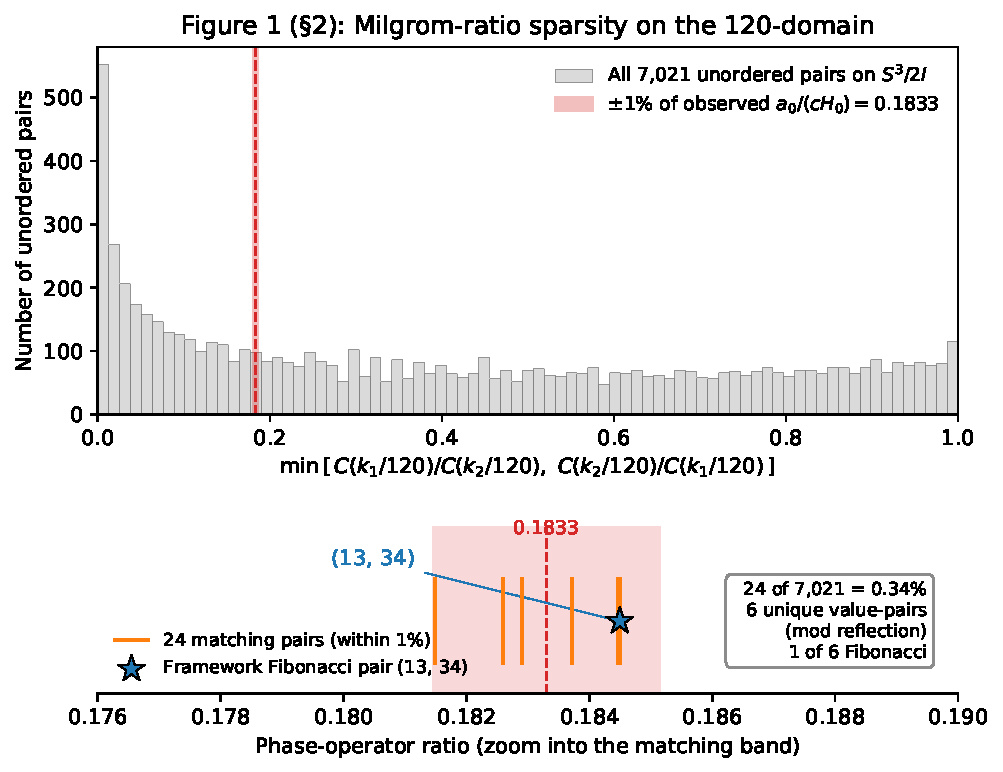
\includegraphics[width=0.85\linewidth]{figure1}
\caption{Milgrom-ratio sparsity on the 120-domain. Of 7,021 unordered
nonzero phase-position pairs, 24 reproduce the observed
$\afid/(cH_0) = 0.1833$ within $1\%$; reflection symmetry $C(k) = C(120-k)$
collapses these to 6 unique phase-operator value pairs. Within the
framework's Fibonacci-well subset $\{13, 21, 34, 55\}/120$, only the
pair $(13, 34)$ matches, marked with a star.}
\label{fig:milgrom-sparsity}
\end{figure}

\paragraph{Local-epoch reading.}
Equation~\eqref{eq:milgrom-ratio-derived} holds at every $z$ because
$N_H(z)$ is calibrated through the local $H(z)$ at the observer's
epoch, not frozen at $N_H(0)$. The alternative, anchoring $N_H$ to the
present, would require a privileged time slice. The bounded domain
$S^3$ with $\partial S^3 = \emptyset$ has no preferred epoch; the
standing wave $\Psi(t) = \cos(t/2)$ that governs the cosmic cycle is
itself $t$-dependent throughout. The local-epoch reading is the
default; freezing $N_H(0)$ would be the addition of a postulate the
topology does not motivate. The two readings are observably distinct at
every $z > 0$: at $z = 2$ the BTFR normalization differs by a factor of
$3$ between them, and the Euclid DR1 test
(Section~\ref{sec:euclid}) will distinguish them.

\paragraph{Why $\Lambda$ does not evolve.} The same scaling law places
$\Lambda$ at the antinode $\Theta = 60/120$ with $n = 2$ (surface
mode), referenced to $\Omega_\Lambda$: the fixed eigenvalue hierarchy
associated with the $\Lambda$ eigenvalue, not the redshift-dependent
fractional density parameter of standard cosmological notation. Under
the local-epoch reading, this eigenvalue hierarchy is the same at every
$z$. The phase position $60/120$ has $d\ln C/d\Theta = 0$, giving
topological protection against perturbation. The two predictions are
structurally inverse: $\afid$ evolves because it references $\Omega_H$;
$\Lambda$ does not because it references $\Omega_\Lambda$. This
inversion is forced by the selection rule (Appendix~\ref{app:selection}).

Thus the result is a conditional prediction of the framework: given
the scaling law, selection rule, calibrated well assignments, and
local-epoch reading, the redshift evolution follows by substitution,
with no additional evolution parameter.


% =====================================================================
\section{Five observable channels}
\label{sec:channels}

The evolution $\afid(z) = \afid(0)\,\Ez$ from
Section~\ref{sec:derivation} propagates into galactic observables
through different powers of $\Ez$. We adopt the flat $\Lambda$CDM
Friedmann form

$\Ez = \sqrt{\Omega_m(1+z)^3 + \Omega_r(1+z)^4 + \Omega_\Lambda}$
with Planck 2018 parameters \citep{Planck2018}
($\Omega_m = 0.315$, $\Omega_r = 9.2 \times 10^{-5}$,
$\Omega_\Lambda = 0.685$, $H_0 = 67.4$~km/s/Mpc). The prediction
$\afid(z) \propto H(z)$ holds for any expansion history; adopting
$\Lambda$CDM is a transparency choice that allows direct comparison
with published measurements. Table~\ref{tab:cosmology} provides the
reference values consumed by the five channels below.

\begin{table}[!ht]
\centering
\caption{Predicted $\afid(z)$ and deep-MOND enhancement factor across
the redshift range relevant to this paper.}
\label{tab:cosmology}
\begin{tabular}{r r r l r r}
\toprule
$z$ & $\Ez$ & $\Hz$~[km/s/Mpc] & $\afid(z)$~[m/s$^2$] & $\sqrt{\Ez}$ & $t_\text{age}$~[Gyr] \\
\midrule
0.0  & 1.000  & 67.4   & $1.20 \times 10^{-10}$ & 1.000 & 13.79 \\
0.5  & 1.322  & 89.1   & $1.59 \times 10^{-10}$ & 1.150 & 8.58  \\
1.0  & 1.791  & 120.7  & $2.15 \times 10^{-10}$ & 1.338 & 5.84  \\
2.0  & 3.033  & 204.4  & $3.64 \times 10^{-10}$ & 1.741 & 3.27  \\
3.0  & 4.568  & 307.9  & $5.48 \times 10^{-10}$ & 2.137 & 2.14  \\
5.0  & 8.297  & 559.2  & $9.96 \times 10^{-10}$ & 2.880 & 1.17  \\
10.0 & 20.53  & 1383   & $2.46 \times 10^{-9}$  & 4.530 & 0.470 \\
15.0 & 36.01  & 2427   & $4.32 \times 10^{-9}$  & 6.001 & 0.268 \\
\bottomrule
\end{tabular}
\end{table}

\subsection{Tully--Fisher normalization: $\Ez^{-1}$}
\label{sec:btfr}

In the deep-MOND limit, the baryonic Tully--Fisher relation (BTFR) is
$\vflat^4 = G\,\Mb\,\afid$ \citep{Lelli2016}. With evolving $\afid$:
\begin{equation}
\boxed{\;\frac{A_\text{BTFR}(z)}{A_\text{BTFR}(0)} = \frac{1}{\Ez}\;},
\qquad A_\text{BTFR} \equiv \frac{1}{G\,\afid}.
\label{eq:btfr}
\end{equation}
The interpolating-function dependence cancels in the ratio: any $\mu(x)$
that fits the local SPARC sample inherits the same fractional
evolution. At fixed baryonic mass, $\vflat(z) = \vflat(0)\,\Ez^{1/4}$;
at fixed velocity, $\Mb(z) = \Mb(0)/\Ez$.

\begin{table}[!ht]
\centering
\caption{BTFR evolution at six reference redshifts.}
\label{tab:btfr}
\begin{tabular}{r r r r}
\toprule
$z$ & $\Ez$ & $A(z)/A(0)$ & $\vflat(z)/\vflat(0)$ at fixed $\Mb$ \\
\midrule
0.0  & 1.000  & 1.000 & 1.000 \\
0.5  & 1.322  & 0.756 & 1.072 \\
1.0  & 1.791  & 0.558 & 1.157 \\
2.0  & 3.033  & 0.330 & 1.320 \\
5.0  & 8.297  & 0.121 & 1.697 \\
10.0 & 20.53  & 0.049 & 2.128 \\
\bottomrule
\end{tabular}
\end{table}

An $L^*$ disk ($\Mb = 6 \times 10^{10}\,\Msun$, $\vflat(0) = 176$~km/s)
is predicted to have $\vflat(z=2) = 232$~km/s, a $32\%$ increase at
fixed baryonic mass. The existing {\"U}bler et~al.\ \citep{Ubler2017} KMOS3D measurement
is the only quantitative test of this prediction; the comparison is
treated in Section~\ref{sec:constraints}.

\subsection{MOND transition radius and asymptotic velocity:
$\Ez^{-1/2}$, $\Ez^{+1/4}$}
\label{sec:rotcurves}

The radius where Newtonian gravity equals $\afid(z)$ is
$\rM = \sqrt{G \Mb / \afid(z)}$, giving
\begin{equation}
\boxed{\;\frac{\rM(z)}{\rM(0)} = \frac{1}{\sqrt{\Ez}}\;}.
\label{eq:rM}
\end{equation}
At $z = 2$, the transition happens at $57\%$ of the local radius. The
asymptotic velocity rises as $\Ez^{1/4}$ (from
Section~\ref{sec:btfr}). Both scalings are mass-independent in the
deep-MOND limit.

\begin{table}[!ht]
\centering
\caption{Predicted MOND radius and asymptotic velocity at $z = 0$ and
$z = 2$ for four SPARC archetypes. The fractional shifts
$\rM(2)/\rM(0) = 0.574$ and $\vflat(2)/\vflat(0) = 1.320$ apply
identically across the table.}
\label{tab:rotcurves}
\resizebox{\linewidth}{!}{%
\begin{tabular}{l r r r r r}
\toprule
Archetype & $\Mb$~[$\Msun$] & $\rM(0)$~[kpc] & $\rM(2)$~[kpc] &
$\vflat(0)$~[km/s] & $\vflat(2)$~[km/s] \\
\midrule
Dwarf (DDO 154)      & $3.5 \times 10^8$    & 0.64  & 0.37 & 49  & 64  \\
Sub-$L^*$ (NGC 2403) & $1.0 \times 10^{10}$ & 3.41  & 1.96 & 112 & 148 \\
$L^*$ (NGC 6946)     & $6.0 \times 10^{10}$ & 8.35  & 4.79 & 176 & 232 \\
Giant (UGC 2885)     & $1.5 \times 10^{11}$ & 13.20 & 7.58 & 221 & 292 \\
\bottomrule
\end{tabular}%
}
\end{table}

The comparison isolates the effect of $\afid(z)$ at fixed baryonic
distribution. Real galaxies at $z = 2$ differ in structural properties;
the observer-facing formulation is: given an observed galaxy at
redshift $z$ with measured $\Mb$ and $\vflat^\text{obs}$, compare
$\vflat^\text{obs}/\Ez^{1/4}$ to the local SPARC value for galaxies of
the same $\Mb$.

\subsection{Lensing dynamical mass: $\Ez^{+1/2}$}
\label{sec:lensing}

Galaxy--galaxy weak lensing infers a dynamical mass
$\Mdyn(R) = \vflat^2 R / G$ within aperture $R$ under the standard
Newtonian inversion. The framework's prediction below applies to this
Newtonian-equivalent proxy, not to a relativistic lensing law it does
not yet supply: it defines the redshift scaling predicted for the
$\Mdyn$ that lensing analyses report under the standard inversion. In
the deep-MOND limit:
\begin{equation}
\boxed{\;\frac{\Mdyn(R,z)/\Mb}{\Mdyn(R,0)/\Mb} = \sqrt{\Ez}\;}.
\label{eq:lensing}
\end{equation}
The enhancement is mass-independent and aperture-independent (for
$R \gg \rM$). At $z = 2$, $\Mdyn/\Mb$ is $74\%$ higher than at $z = 0$
at any fixed mass and aperture (Figure~\ref{fig:lensing-discriminator}).

\begin{figure}[!ht]
\centering
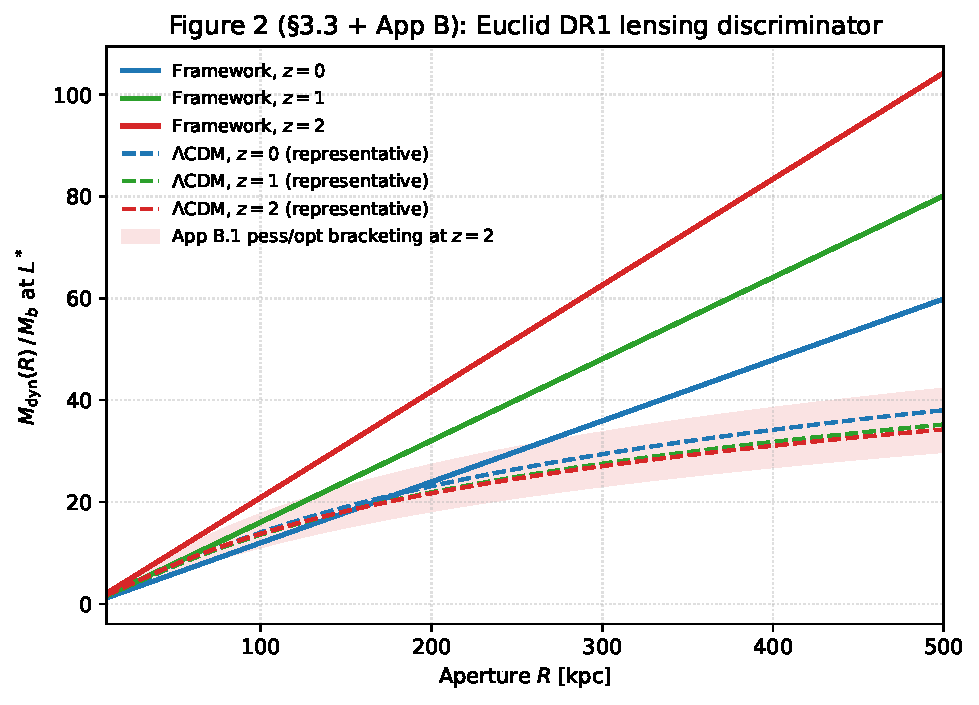
\includegraphics[width=0.85\linewidth]{figure2}
\caption{Euclid DR1 lensing discriminator. Framework prediction
(universal $\sqrt{\Ez}$ enhancement, dashed) versus $\Lambda$CDM
prediction (mass- and aperture-dependent, solid bands) for $\Mdyn/\Mb$
across galaxy stellar-mass strata at the canonical $R = 100$~kpc
aperture. The framework predicts a single $1.74$ enhancement factor at
$z = 2$ across all masses; $\Lambda$CDM spans 37 percentage points
across the SPARC archetype range.}
\label{fig:lensing-discriminator}
\end{figure}

\begin{table}[!ht]
\centering
\caption{Predicted $\Mdyn/\Mb$ for the $L^*$ archetype at three lensing
apertures.}
\label{tab:lensing}
\begin{tabular}{r r r r r r}
\toprule
$R$~[kpc] & $z = 0$ & $z = 0.5$ & $z = 1$ & $z = 2$ & $z = 5$ \\
\midrule
30  & 3.59  & 4.13  & 4.81  & 6.26  & 10.35  \\
100 & 11.98 & 13.77 & 16.03 & 20.86 & 34.50  \\
300 & 35.93 & 41.32 & 48.08 & 62.57 & 103.50 \\
\bottomrule
\end{tabular}
\end{table}

Under $\Lambda$CDM, halo concentration evolution produces $\Mdyn/\Mb$
shifts that depend on both mass and aperture
\citep{Moster2013,Duffy2008}. The framework predicts a universal
$\sqrt{\Ez}$ factor across all masses and apertures. A Euclid DR1
stacked analysis stratified by both galaxy stellar mass and aperture
tests the magnitude and the universality of the prediction in a single
dataset (Section~\ref{sec:euclid}).

\subsection{Collapse time: $\Ez^{-1/4}$ (supporting evidence)}
\label{sec:collapse}

In the deep-MOND regime, $\geff = \sqrt{\gN \cdot \afid(z)}$ scales as
$\sqrt{\Ez}$ at fixed source, and the free-fall time
$\tff \propto 1/\sqrt{\geff}$ shortens as $\Ez^{-1/4}$. At $z \sim 8$,
the factor $\Ez^{1/4} \approx 2$ shortens the characteristic deep-MOND
collapse time by approximately a factor of two. This eases, but does
not by itself resolve, the star-formation-efficiency pressure for the
Labb{\'e} et~al.\ \citep{Labbe2023} massive candidates. Whether this resolves the
impossibility constraint for any specific candidate depends on
halo-mass priors the framework does not modify; the per-object analysis
is reserved for future work. The fourth-root dependence makes this
channel robust: a $10\%$ shift in $\Ez$ changes the correction by less
than $3\%$.

\subsection{Summary: five exponents from one input}
\label{sec:five-exponents}

\begin{table}[!ht]
\centering
\caption{The full predictive content of the evolving acceleration
scale, evaluated at $z = 2$.}
\label{tab:five-exponents}
\small
\setlength{\tabcolsep}{4pt}
\begin{tabular}{l l r l}
\toprule
Observable & Scaling & Value at $z = 2$ & Primary test \\
\midrule
BTFR normalization                 & $\Ez^{-1}$    & 0.330 & Euclid DR1, KMOS3D \\
MOND radius                         & $\Ez^{-1/2}$  & 0.574 & High-$z$ rotation curves \\
Asymptotic velocity at fixed $\Mb$ & $\Ez^{+1/4}$  & 1.320 & Euclid DR1, KMOS3D \\
Lensing $\Mdyn/\Mb$                & $\Ez^{+1/2}$  & 1.741 & Euclid DR1 stacked lensing \\
Free-fall collapse time             & $\Ez^{-1/4}$  & 0.758 & JWST spectroscopy \\
\bottomrule
\end{tabular}
\end{table}

\begin{figure}[!ht]
\centering
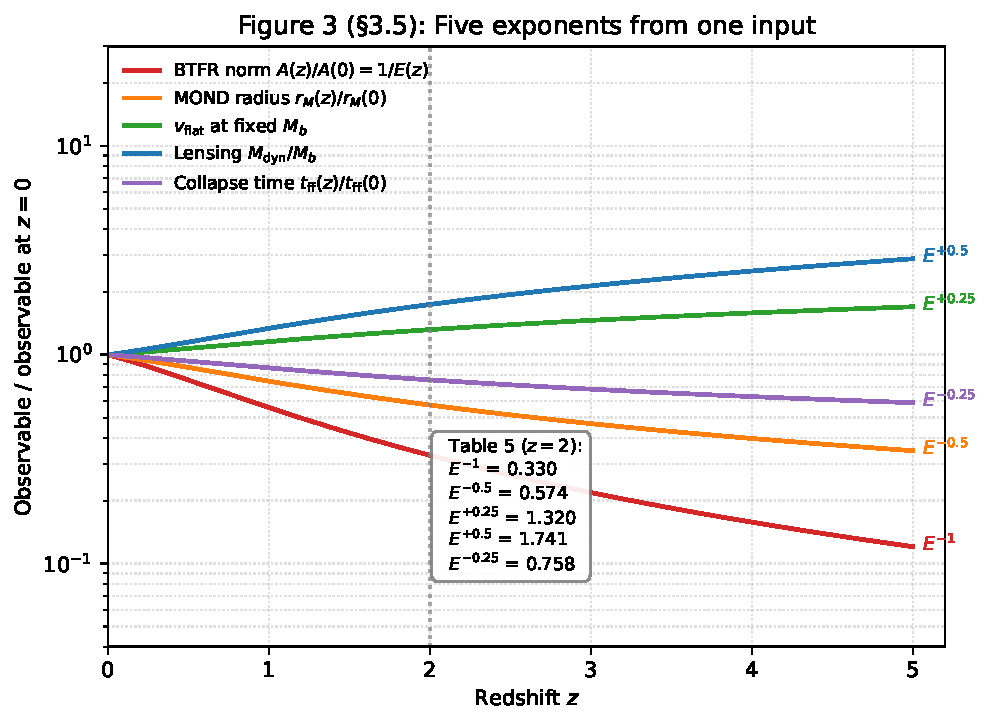
\includegraphics[width=0.85\linewidth]{figure3}
\caption{Five exponents from one input. Each curve plots the predicted
fractional shift in one observable as a function of redshift, derived
from the single relation $\afid(z) = \afid(0)\,\Ez$. Consistency across
channels at the same $z$ tests the universality of the deep-MOND
scaling.}
\label{fig:five-exponents}
\end{figure}

The five exponents are correlated manifestations of one input
(Figure~\ref{fig:five-exponents}): any single channel tests
$\afid(z) = \afid(0)\,\Ez$, and agreement among channels at one redshift
tests whether the deep-MOND scaling is universal.

% =====================================================================
\section{Existing constraints}
\label{sec:constraints}

\subsection{The {\"U}bler tension}
\label{sec:ubler}

The KMOS3D analysis of {\"U}bler et~al.\ \citep{Ubler2017} is the only existing
quantitative test of the Section~\ref{sec:btfr} prediction at
intermediate redshift. Their fixed-slope BTFR zero-point offsets
relative to the local Lelli et~al.\ \citep{Lelli2016} baseline are
\begin{equation*}
\Delta b^{\text{obs}}(z{=}0.9) = -0.44 \pm 0.04~\text{dex},
\qquad
\Delta b^{\text{obs}}(z{=}2.3) = -0.27 \pm 0.05~\text{dex}.
\end{equation*}
The framework predicts
\begin{equation*}
\Delta b^{\text{MIT}}(z{=}0.9) = -0.227~\text{dex},
\qquad
\Delta b^{\text{MIT}}(z{=}2.3) = -0.540~\text{dex}.
\end{equation*}
The magnitudes overlap: both the prediction and the data place the
high-$z$ BTFR substantially below the local relation. The trend shapes
do not: the data are non-monotonic ($-0.44 \to -0.27$), the prediction
strictly monotonic ($-0.227 \to -0.540$) (Figure~\ref{fig:ubler}).

\begin{figure}[!ht]
\centering
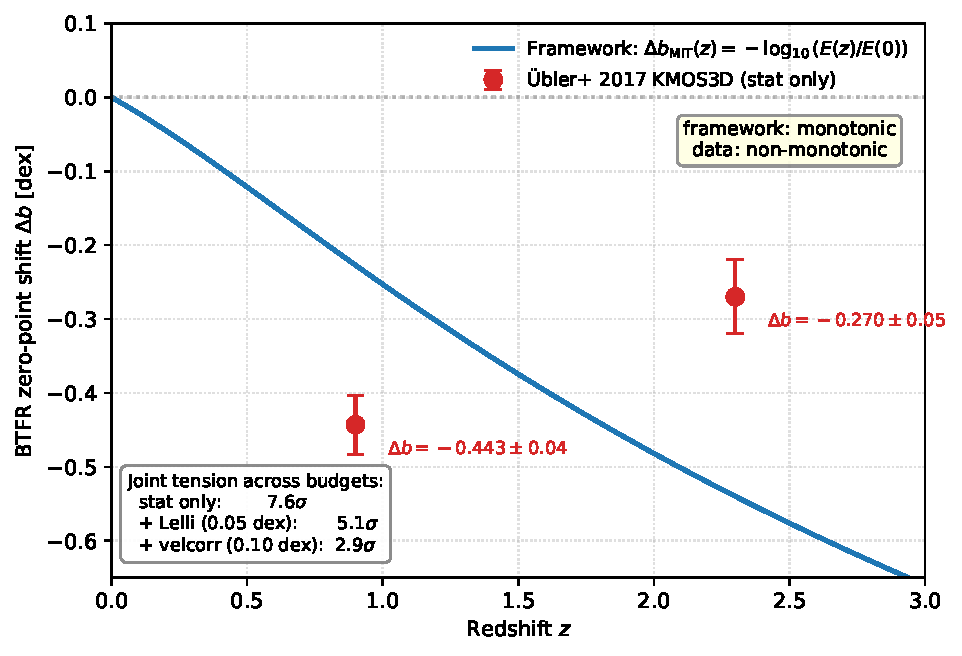
\includegraphics[width=0.85\linewidth]{figure4}
\caption{KMOS3D BTFR trend-shape tension. The framework predicts a
strictly monotonic decrease (dashed); the {\"U}bler et~al.\ \citep{Ubler2017} data are
non-monotonic. The joint tension is 2.9$\sigma$ under the most
conservative systematics budget.}
\label{fig:ubler}
\end{figure}

\newpage

The tension is quantified across three uncertainty budgets:

\begin{table}[!ht]
\centering
\caption{Per-bin and joint $\sigma$-tension for the KMOS3D BTFR comparison
under three uncertainty budgets.}
\label{tab:sigma-tension}
\begin{tabular}{l r r r}
\toprule
Budget & $T(z{=}0.9)$~[$\sigma$] & $T(z{=}2.3)$~[$\sigma$] & Joint~[$\sigma$] \\
\midrule
{\"U}bler statistical only         & $-5.4$ & $+5.4$ & 7.6 \\
$+$ local-baseline ($0.05$~dex)    & $-3.4$ & $+3.8$ & 5.1 \\
$+$ velocity-correction ($0.10$~dex) & $-1.8$ & $+2.2$ & 2.9 \\
\bottomrule
\end{tabular}
\end{table}

Even under the most conservative budget, the joint tension is
$2.9\sigma$. We treat this as a provisional tension rather than a
formal falsification, because the comparison combines heterogeneous
velocity definitions and cross-redshift pressure-support corrections.
Formal falsification requires a matched-systematics measurement: single
instrument, uniform tracer, identical correction prescription across
redshift bins (Section~\ref{sec:euclid}).

We tested whether the {\"U}bler radial pressure-support correction can
produce the observed non-monotonic pattern from a monotonic underlying
BTFR. Mock galaxies at $z = 0.9$ and $z = 2.3$ were generated under the
framework's prediction with literature-realistic distributions of
baryonic mass, scale length, and velocity dispersion
\citep{Wisnioski2015}. The {\"U}bler thick-disk correction
$v_\text{circ}^2(r) = v_\text{rot}^2(r) + 2\sigma_0^2\,r/R_d$ was
applied with the published selection cut
$v_\text{rot,max}/\sigma_0 > 4.4$. Four bias models (radial-position
uncertainty, beam-smearing of $\sigma_0$, non-asymptotic rotation
curves, selection-induced mass shifts) were swept over
literature-plausible ranges. No combination reproduces the observed
$(-0.44, -0.27)$ pattern. Pulling biases to optimize the $z = 0.9$ fit
gives $\Delta b(0.9) = -0.29$~dex, leaving the $z = 0.9$ point
$0.15$~dex above observed; at the same parameters
$\Delta b(2.3) = -0.65$~dex, $0.38$~dex below observed. The joint-L2
best fit gives $(\Delta b(0.9), \Delta b(2.3)) = (-0.17, -0.43)$ at
residuals $(+0.28, -0.16)$~dex. The mock-generation script, bias
parameterization, and random seeds are archived with the rest of the
analysis pipeline at the Zenodo deposit cited in the Data availability
section.


The pattern is not a velocity-correction artifact. The
prediction stands. Resolution will come from Euclid DR1 stacked lensing
and JWST/ground-IFU matched-tracer follow-up at the original {\"U}bler
redshifts (Section~\ref{sec:euclid}).

\subsection{Galaxy clusters}
\label{sec:clusters}

MOND analyses of local galaxy clusters \citep{Pointecouteau2005} report
a residual mass discrepancy of roughly a factor of $5$ at
$r \approx 0.5\,\Rvir$. The framework's evolving $\afid$ does not
address this: the relevant clusters sit at $z \lesssim 0.15$, where
$\Ez \leq 1.08$ and the framework correction is less than $8\%$. A
factor-of-$5$ problem is not touched by an $8\%$ correction. This
discrepancy is an open problem shared by all MOND-class theories
\citep{Sanders2003,Angus2008,Famaey2012} and predates the present
framework, which neither introduces nor resolves it.

\newpage

\subsection{The CMB at recombination}
\label{sec:cmb}

A naive application of $\afid(z)$ to cosmological perturbations at
$z = 1090$ gives $\afid \approx 23{,}000 \times \afid(0)$, placing
recombination-scale perturbations deep in the MOND regime and
disrupting the acoustic peak structure that Planck fits at sub-percent
precision.

The framework's selection rule (Section~\ref{sec:derivation},
Appendix~\ref{app:selection}) separates this channel structurally. The
rule assigns $\afid$ to the edge sector ($n = 1$, $\Omega_H$) and
cosmological perturbations to the space sector ($n = 3$,
$\Omega_\Lambda$). Under this assignment, the $\afid(z)$ scaling
governs galactic dynamics and does not propagate to perturbation
evolution. The same rule independently produces the
Section~\ref{sec:derivation} Milgrom-ratio match at $0.7\%$ and the
$\Lambda$-constant prediction; it was not introduced to address the
CMB.

The consistency condition is quantitative. Writing a minimal leakage
coupling $\geff = \gN + \varepsilon\sqrt{\gN\,\afid(z)}$, the Planck
first-peak amplitude, measured to $0.5\%$ precision, constrains
$\varepsilon \leq 1.2 \times 10^{-5}$. The framework predicts
$\varepsilon = 0$ under exact edge/space decoupling, satisfying the
bound by five orders of magnitude. A first-principles perturbation-theory
derivation of the decoupling is the principal open task for the
framework's CMB-scale predictions.

\subsection{Other regimes}
\label{sec:other-regimes}

Local SPARC and THINGS measurements are consistent by construction: the
well assignments were calibrated against $\afid(0)$ and $H_0$ at
$z = 0$ (Section~\ref{sec:derivation}). The Genzel et~al.\ \citep{Genzel2017}
SINS/zC-SINF sample of six massive star-forming disks at
$z = 0.9$--$2.4$ reports declining outer rotation curves with low
inferred dark-matter fractions; because no fixed-slope BTFR zero-point
is published, the data are qualitatively consistent with
Section~\ref{sec:btfr} but do not provide a quantitative test of the
normalization prediction. Strong-lensing time-delay cosmography
(TDCOSMO~\citep{Millon2020}, H0LiCOW~\citep{Wong2020}) is below current
sensitivity to the framework's predictions. None of these regimes is
sharp enough to test the framework's normalization prediction
independently.

\subsection{Summary}
\label{sec:constraint-summary}

\begin{table}[!ht]
\centering
\caption{Constraint status across five regimes.}
\label{tab:constraint-status}
\small
\begin{tabular}{p{0.32\linewidth} p{0.60\linewidth}}
\toprule
Regime & Status \\
\midrule
Local ($z = 0$)                        & Consistent by construction \\
Intermediate-$z$ BTFR ({\"U}bler~\citep{Ubler2017}) & $2.9\sigma$ tension on trend shape \\
Galaxy clusters~\citep{Pointecouteau2005}          & Inherited, unaddressed ($\sim 8\%$ vs factor-5) \\
CMB ($z = 1090$)                       & Structurally decoupled; $\varepsilon \leq 1.2 \times 10^{-5}$ from Planck \\
Strong-lens time delays                & Below current sensitivity \\
\bottomrule
\end{tabular}
\end{table}

One live tension, one inherited problem, one structural decoupling, two
consistencies. The {\"U}bler tension is held against the prediction
without retreat.


% =====================================================================
\section{The Euclid DR1 test}
\label{sec:euclid}

Euclid's stated objective is to characterize the dark Universe and its
evolution across $z = 0$--$2$ \citep{Euclid2024}. The present paper
focuses on the galactic-dynamics prediction
$\afid(z) \propto H(z)$. The Euclid DR1 release in October 2026 is
expected to deliver the sharpest test of this prediction through
stacked galaxy--galaxy weak lensing at $z = 0.5$--$2$.

\paragraph{What Euclid measures.}
The wide survey is expected to provide the photometric redshifts,
stellar-mass estimates, galaxy shapes, and sample sizes needed for a
stacked galaxy--galaxy lensing test. For the framework, the relevant
observable is the Newtonian-equivalent $\Mdyn/\Mb$ inferred from
stacked tangential shear profiles after mass and redshift
stratification. Equation~\eqref{eq:lensing} is a prediction for this
quoted proxy, not a standalone relativistic lensing law.

\paragraph{What the framework predicts.}
At fixed baryonic mass and aperture, $\Mdyn/\Mb$ is enhanced by
$\sqrt{\Ez}$ relative to $z = 0$: a $15\%$ excess at $z = 0.5$, $34\%$
at $z = 1$, and $74\%$ at $z = 2$ (Table~\ref{tab:lensing}). The
enhancement is universal across galaxy mass and lensing aperture in the
deep-MOND regime.

\paragraph{Why this discriminates from $\Lambda$CDM.}
Under $\Lambda$CDM, $\Mdyn/\Mb$ also evolves with redshift through halo
concentration evolution and stellar-to-halo mass relation shifts
\citep{Moster2013,Duffy2008}. The $\Lambda$CDM prediction is
mass-dependent and aperture-dependent: at $z = 2$ relative to $z = 0$,
the $\Lambda$CDM ratio shifts by a factor of $0.76$ for a Sub-$L^*$
galaxy, $0.98$ for $L^*$, and $1.13$ for a Giant at the canonical
$R = 100$~kpc aperture, spanning 37 percentage points across the mass
range (Appendix~\ref{app:lensing}). The framework predicts the same
factor $1.74$ for all three. A Euclid DR1 analysis stratified by both
stellar mass and aperture tests the magnitude and the universality of
the prediction in a single dataset.

\paragraph{Falsification criteria.}

\begin{table}[!ht]
\centering
\caption{Falsification criteria for the five Section~\ref{sec:channels}
predictions. A matched-systematics discrepancy at $\geq 2\sigma$ is
treated as a reportable tension; formal falsification requires either
$\geq 3\sigma$ in one channel or mutually consistent $\geq 2\sigma$
failures across independent redshift bins or observables.}
\label{tab:falsification}
\footnotesize
\setlength{\tabcolsep}{3pt}
\begin{tabular}{p{0.16\linewidth} p{0.21\linewidth} p{0.32\linewidth} p{0.20\linewidth}}
\toprule
Prediction & Signature & Reportable tension if & Key systematic \\
\midrule
BTFR normalization & $A(z)/A(0) = 1/\Ez$ & Single-$z$ inconsistency at $\geq 2\sigma$ & Pressure-support correction \\
BTFR trend shape & Monotonic decrease & Non-monotonic trend confirmed under matched systematics & Cross-instrument tracer mismatch \\
MOND radius & $\rM(z)/\rM(0) = \Ez^{-1/2}$ & Single-$z$ inconsistency at $\geq 2\sigma$ & Baryonic mass model \\
Lensing enhancement & $\sqrt{\Ez}$, mass/aperture-independent & Inconsistency at $\geq 2\sigma$, or mass/aperture-dependent shift & Halo concentration evolution \\
Collapse-time correction & $\tff(z)/\tff(0) = \Ez^{-1/4}$ & Corrected formation timescales incompatible with spectroscopic ages at $\geq 2\sigma$ & Halo-mass priors \\
\bottomrule
\end{tabular}
\end{table}

The lensing row is the cleanest because $\sqrt{\Ez}$ is universal while
the $\Lambda$CDM alternative is not. A mass- and aperture-stratified
Euclid analysis tests both the magnitude of the prediction and its
universality simultaneously.

\begin{table}[!ht]
\centering
\caption{Near-term test schedule.}
\label{tab:schedule}
\footnotesize
\setlength{\tabcolsep}{3pt}
\begin{tabular}{p{0.26\linewidth} p{0.22\linewidth} p{0.32\linewidth} p{0.13\linewidth}}
\toprule
Window & Instrument & Tests & Delivery \\
\midrule
Stacked lensing, $z = 0.5$--$2$            & Euclid DR1                    & Lensing enhancement, universality        & October 2026 \\
Emission-line sample selection             & Euclid NISP grism             & Lens sample definition, redshift binning & October 2026 \\
Matched-tracer BTFR                        & JWST NIRSpec IFU / ground IFU & BTFR normalization, trend shape          & In progress  \\
Resolved kinematics at {\"U}bler redshifts & JWST NIRSpec IFU              & BTFR at $z = 0.9$, $z = 2.3$             & In progress  \\
Spectroscopic confirmation, $z = 7$--$9$   & JWST NIRSpec                  & JWST efficiency                          & 2025--2026   \\
\bottomrule
\end{tabular}
\end{table}

All programs listed are existing or imminent. No new instrument or
observational capability is required. This paper and its predictions
are deposited on Zenodo (concept DOI:
\href{https://doi.org/10.5281/zenodo.19980665}{10.5281/zenodo.19980665})
prior to the Euclid DR1 release, fixing the numbers before the data
arrive.

% =====================================================================
\section{Conclusions}
\label{sec:conclusions}

The Milgrom coincidence $\afid \approx cH_0$ is accounted for, within
the bounded-topology framework of Appendix~\ref{app:framework}, by a
fixed ratio of two phase-operator values at Fibonacci wells:
$\afid/(cH) = \Cval{13}/\Cval{34} = 0.1845$, agreeing with the observed
$0.1833$ at $0.7\%$. The $\afid$ and $H$ wells are fixed by separately
calibrated assignments at $z = 0$ sharing the same edge-mode hierarchy;
the ratio follows algebraically and is unique among the framework's
Fibonacci-well pairs (Section~\ref{sec:derivation}).

Because both observables reference the same epoch-dependent hierarchy,
the ratio holds at every cosmic epoch:
$\afid(z) = \afid(0)\,\Ez$. Five observable channels follow as
different powers of $\Ez$, with no additional free parameter. The BTFR
normalization shifts as $\Ez^{-1}$, the MOND transition radius
contracts as $\Ez^{-1/2}$, the asymptotic velocity at fixed baryonic
mass rises as $\Ez^{+1/4}$, the lensing-inferred dynamical mass
enhancement scales as $\Ez^{+1/2}$, and the gravitational collapse time
shortens as $\Ez^{-1/4}$. The five exponents move together, set by one
input; cross-channel agreement at a fixed redshift is the test of the
deep-MOND scaling.

The prediction lives in a constraint landscape with one tension
({\"U}bler et al.\ KMOS3D BTFR trend shape at $2.9\sigma$, tested by
forward modeling), one inherited problem
(cluster-scale MOND discrepancy, untouched by the framework's
$\lesssim 8\%$ low-redshift correction), and one structural decoupling
(CMB via the selection rule, with leakage bounded to
$\varepsilon \leq 1.2 \times 10^{-5}$ by Planck). The {\"U}bler tension
is acknowledged, not explained away.

A separate preprint applies the same selection rule to the dark-energy
sector
(DOI:~\href{https://doi.org/10.5281/zenodo.19798852}{10.5281/zenodo.19798852});
the present paper is limited to the galactic-dynamics consequence
$\afid(z) = \afid(0)\,\Ez$.

The sharpest scheduled test is Euclid DR1 in October 2026: stacked
galaxy--galaxy lensing at $z = 0.5$--$2$ stratified by mass and
aperture, probing both the predicted $74\%$ enhancement and its
universality in a regime where the framework and $\Lambda$CDM produce
quantitatively distinct shifts. This paper and its predictions are
deposited on Zenodo (concept DOI:
\href{https://doi.org/10.5281/zenodo.19980665}{10.5281/zenodo.19980665})
prior to that release.

% =====================================================================
\appendix
\renewcommand{\thesection}{\Alph{section}}
\renewcommand{\theequation}{\thesection.\arabic{equation}}
\renewcommand{\thetable}{\thesection.\arabic{table}}
\renewcommand{\thefigure}{\thesection.\arabic{figure}}
\setcounter{equation}{0}
\setcounter{table}{0}
\setcounter{figure}{0}

% =====================================================================
\section{Framework foundations}
\label{app:framework}

This appendix supplies the structural detail behind the
Section~\ref{sec:derivation} derivation. The bounded topology, phase
operator, scaling law, and selection rule are stated in
Section~\ref{sec:derivation}. This appendix develops the 120-domain
(\ref{app:120-domain}), the selection rule's physical basis
(\ref{app:selection}), and the well-assignment eligibility conditions
(\ref{app:wells}).

\subsection{The 120-domain}
\label{app:120-domain}

The physical observable space is the quotient $S^3/2I$, where $2I$ is
the binary icosahedral group with $|2I| = 120$. The discrete subgroups
of $\text{SU}(2) \cong S^3$ are classified: cyclic groups
$\mathbb{Z}_n$, binary dihedral groups $2D_n$, and three exceptional
groups (binary tetrahedral $|2T| = 24$, binary octahedral $|2O| = 48$,
binary icosahedral $|2I| = 120$). Two constraints select $2I$.

The quotient $S^3/2I$ is the Poincar{\'e} homology sphere: the
classical example of a closed 3-manifold with the integral homology of
$S^3$ but nontrivial fundamental group, obtained as the quotient of
$S^3$ by the binary icosahedral group $2I$ \citep{Saveliev2012}. The
same group occupies the $E_8$ position in the ADE classification of
finite subgroups of $\text{SU}(2)$, and its representation theory maps
to the $E_8$ Dynkin diagram through the McKay correspondence
\citep{McKay1980}. More generally, quotients $S^3/\Gamma$ by finite
freely acting subgroups are spherical space forms, classified in the
standard space-form literature \citep{Wolf2011}. The framework's use of
$2I$ is therefore not ad hoc: within the finite exceptional binary
polyhedral subgroups of $\text{SU}(2)$, it is the largest case and the
$E_8$ endpoint of the ADE/McKay classification.

First, $2I$ is the largest exceptional discrete subgroup of
$\text{SU}(2)$, giving the maximum spectral resolution compatible with
$S^3$. In the framework, the quotient order $|2I| = 120$ defines the
discrete phase domain used to label observable positions, with spacing
$\Delta\Theta = 1/120$.

Second, the icosahedron is the unique Platonic solid whose branch
orders $(2, 3, 5)$ are consecutive Fibonacci numbers satisfying
$2 + 3 = 5$. This Fibonacci-recurrence structure makes the Fibonacci
positions on the 120-domain the natural stable lattice
(\ref{app:selection} below and the Hurwitz stability argument in
\ref{app:wells}).

The phase position is quantized:
$\Theta \in \{k/120 : k = 0, 1, \ldots, 119\}$. For photon-mediated
observables, the bosonic projection $|\psi|^2$ erases the
anti-periodic sign flip, halving the resolution to a 60-position grid
(even numerators only). The framework implements this as a bosonic
projection: photon-mediated observables sample the 60-position
quotient, while dynamical observables may access the full 120-domain.

The chronon, the smallest phase advance the domain can register, is
$\Delta t_\text{min} = 4\pi/120 = \pi/30$, giving a minimum action
$\Delta S_\text{min} = \hbar\pi/30$ that is frame-independent by
construction.

\subsection{The selection rule}
\label{app:selection}

The scaling law (Section~\ref{sec:derivation},
Eq.~\ref{eq:scaling-law}) assigns each observable a manifold-mode index
$n$ from the embedding hierarchy $S^1 \subset \Mob \subset S^3$ and a
corresponding hierarchy normalization $N$. The physical basis for the
$(n, \Omega)$ assignment is:

\paragraph{Edge modes ($n = 1$, $\Omega_H$).}
The boundary $S^1$ is a kinematic locus: it carries no intrinsic
eigenvalue (the surface eigenvalue lives one dimension up, on the
\Mob{} strip, where $\Lambda$ is placed). What an edge-mode observable
references is the embedding scale of $S^1$ in the ambient cosmological
geometry. The natural such scale is the Hubble horizon $R_H = c/H$, and
its dimensionless Planck ratio is $\Omega_H = (c/(H\ell_P))^2$. Because
$H$ evolves with cosmic epoch, edge-mode observables inherit that
evolution through the calibrated normalization
$N_H(z) = H(z)\,t_P/\Cval{34}$.

\paragraph{Surface modes ($n = 2$, $\Omega_\Lambda$).}
The \Mob{} strip carries an intrinsic eigenvalue: the ground mode of
the Laplace--Beltrami operator on the totally geodesic surface in $S^3$
gives $\lambda_0 = 2/R^2$, where $R$ is the curvature radius of $S^3$.
The Gauss--Codazzi embedding converts this to
$\Lambda_\text{obs} = (3/2)\lambda_0 = 3/R^2$ under three conditions:
totally geodesic embedding ($K_{ij} = 0$), isotropy (CMB-verified to
$10^{-5}$), and de Sitter vacuum. The hierarchy ratio
$\Omega_\Lambda = (\Lambda\ell_P^2)^{-1}$ is set by this eigenvalue and
does not evolve.

\paragraph{Space modes ($n = 3$, $\Omega_\Lambda$).}
Cosmological perturbations propagate on the spatial slice $S^3$ and
reference the same fixed eigenvalue hierarchy as the surface. Under
this assignment, perturbation evolution is governed by $\Omega_\Lambda$,
not $\Omega_H$, and inherits no $\afid(z)$ modification. This is the
structural basis for the CMB consistency argument in
Section~\ref{sec:cmb}.

\subsection{Well assignments}
\label{app:wells}

Three eligibility conditions determine which Fibonacci wells are
consistent with each observable:

\begin{enumerate}[label=\textbf{\arabic*.}, leftmargin=*]
\item \textbf{Manifold index} separates edge modes ($n = 1$: $H_0$,
$\afid$) from surface modes ($n = 2$: $\Lambda$).

\item \textbf{Bosonic projection.} Photon-mediated observables access
only the 60-grid (even numerators); dynamical observables access the
full 120-grid.

\item \textbf{Antinode requirement.} $\Lambda$, as a topologically
protected eigenvalue, sits at $\Theta = 60/120$ where
$d\ln C/d\Theta = 0$.
\end{enumerate}

The Fibonacci wells on the 120-domain are $\{13, 21, 34, 55\}/120$,
corresponding to $F_7$ through $F_{10}$. The lower bound $F_7 = 13$ is
the noise floor: below this, the amplitude $C(k/120)$ is
indistinguishable from neighboring positions. The upper bound
$F_{10} = 55$ is set by the reflection symmetry $C(k) = C(120 - k)$,
which makes $F_{11} = 89$ equivalent to $F_8 = 21$. These bounds are
motivated by the Hurwitz stability criterion: $\varphi$ is the
irrational hardest to approximate by rationals of bounded denominator,
so Fibonacci positions on the 120-domain are taken to minimize
destructive interference between modes.

Under the eligibility conditions:

\begin{enumerate}[label=(\alph*), leftmargin=*]
\item $\afid$ is assigned $\Theta = 13/120$: the unique coprime
position ($\gcd(13, 120) = 1$), accessible only on the full 120-grid as
required for a dynamical (non-photon-mediated) observable.

\item $H_0$ is assigned $\Theta = 34/120$: the unique even-numerator
Fibonacci well among $13/120$, $21/120$, $34/120$, and $55/120$,
consistent with the bosonic-projection condition for a photon-mediated
observation.

\item $\Lambda$ is assigned $\Theta = 60/120$: the antinode, where the
phase operator takes its maximum and the log-slope vanishes.
\end{enumerate}

The wells $21/120$ and $55/120$ remain unassigned in this paper. The
assignments have the status of empirical calibrations at $z = 0$ that
land on positions compatible with the eligibility conditions. The
manifold-mode classification, bosonic-projection filter, selection
rule, and the prediction $\afid(z) \propto H(z)$ were established in
the framework's foundational deposit \citep{Shatto2025} prior to the
present paper's calibration, foreclosing post-hoc adjustment of the
eligibility conditions to fit the well assignments. A first-principles
derivation from the Hurwitz/Fibonacci structure of the 120-domain is
future work.

% =====================================================================
\section{$\Lambda$CDM lensing comparison methodology}
\label{app:lensing}

Section~\ref{sec:lensing} and Section~\ref{sec:euclid} compare the
framework's universal $\sqrt{\Ez}$ lensing enhancement against the
$\Lambda$CDM prediction under halo concentration evolution. This
appendix specifies the parameterization.

\subsection{Galaxy archetypes and halo parameters}
\label{app:archetypes}

Four baryonic-mass archetypes span the SPARC range:

\begin{table}[!ht]
\centering
\caption{Baryonic-mass archetypes spanning the SPARC range.}
\label{tab:archetypes}
\begin{tabular}{l r}
\toprule
Archetype & $\Mb$~[$\Msun$] \\
\midrule
Dwarf (DDO 154)      & $3.5 \times 10^8$    \\
Sub-$L^*$ (NGC 2403) & $1.0 \times 10^{10}$ \\
$L^*$ (NGC 6946)     & $6.0 \times 10^{10}$ \\
Giant (UGC 2885)     & $1.5 \times 10^{11}$ \\
\bottomrule
\end{tabular}
\end{table}

Representative halo masses and concentrations at the $L^*$ archetype,
consistent with the Moster et~al.\ \citep{Moster2013} stellar-to-halo mass relation and
the Duffy et~al.\ \citep{Duffy2008} concentration evolution:

\begin{table}[!ht]
\centering
\caption{Representative halo masses and concentrations at the $L^*$
archetype.}
\label{tab:halo-params}
\begin{tabular}{r r r}
\toprule
$z$ & $\Mhalo$~[$\Msun$] & $c$ \\
\midrule
0 & $1.5 \times 10^{12}$ & 7.5 \\
1 & $1.0 \times 10^{12}$ & 5.0 \\
2 & $7.0 \times 10^{11}$ & 3.5 \\
\bottomrule
\end{tabular}
\end{table}

Sub-$L^*$ and Giant archetypes use mass-appropriate $(\Mhalo, c)$
values from the same parameterization. The SHMR mapping is used only
to set representative halo masses; the discriminator depends on the
relative mass- and aperture-dependence of the $\Lambda$CDM prediction,
not the absolute baryonic-to-halo normalization. These are
representative defaults; alternative SHMR inversions shift the absolute
$\Lambda$CDM values but preserve the mass- and aperture-dependence
that constitutes the Section~\ref{sec:euclid} discriminator.

\subsection{NFW enclosed mass}
\label{app:nfw}

The dynamical mass at fixed physical aperture $R$ is
\begin{equation*}
\Mdyn(R, z) = \NFW(R; \Mhalo, c, z) + \Mb,
\end{equation*}
with NFW enclosed mass
\begin{equation*}
\NFW(R) = \Mhalo \cdot
\frac{\ln(1 + R/r_s) - (R/r_s)/(1 + R/r_s)}{\ln(1 + c) - c/(1 + c)},
\end{equation*}
scale radius $r_s = \Rvir/c$, and virial radius under the $R_{200}$
convention:
\begin{equation*}
\Rvir^3 = \frac{3\,\Mhalo}{4\pi \cdot 200 \cdot \rhocrit(0)\,\Ez^2}.
\end{equation*}
The ratio $\Mdyn/\Mb$ is computed under the same Newtonian inversion
used by the framework prediction (Section~\ref{sec:lensing},
Eq.~\ref{eq:lensing}).

\subsection{The discriminator}
\label{app:discriminator}

At the canonical $R = 100$~kpc aperture, the $\Lambda$CDM $\Mdyn/\Mb$
ratio at $z = 2$ relative to $z = 0$ is:

\begin{table}[!ht]
\centering
\caption{$\Lambda$CDM $\Mdyn/\Mb$ ratio at $z = 2$ relative to $z = 0$,
versus the framework's universal prediction.}
\label{tab:lcdm-archetypes}
\begin{tabular}{l r r}
\toprule
Archetype & $\Lambda$CDM ratio ($z{=}2$/$z{=}0$) & Framework ratio \\
\midrule
Sub-$L^*$ & 0.76 & 1.74 \\
$L^*$     & 0.98 & 1.74 \\
Giant     & 1.13 & 1.74 \\
\bottomrule
\end{tabular}
\end{table}

The $\Lambda$CDM prediction spans 37 percentage points across the mass
range ($0.76$ to $1.13$); the framework predicts a universal $1.74$. At
fixed $L^*$ mass, the $\Lambda$CDM ratio also varies with aperture:
$1.07$ at $R = 30$~kpc, $0.98$ at $R = 100$~kpc, $0.92$ at
$R = 300$~kpc; the framework predicts $1.74$ at all three.

\paragraph{Sensitivity bracketing.}
Table~\ref{tab:bracketing} evaluates the same NFW pipeline under
pessimistic and optimistic SHMR $+$ concentration parameterizations at
the $L^*$ archetype, $R = 100$~kpc.

\begin{table}[!ht]
\centering
\caption{$\Lambda$CDM $L^*$ $\Mdyn/\Mb$ at $R = 100$~kpc under three
parameterizations, against the framework's universal prediction.}
\label{tab:bracketing}
\resizebox{\linewidth}{!}{%
\begin{tabular}{@{}l c c c c@{}}
\toprule
Parameterization & $(\Mhalo, c)$ at $z = 0$ & $(\Mhalo, c)$ at $z = 2$
                & \shortstack{$\Mdyn/\Mb$\\ $z=0$ / $z=2$}
                & \shortstack{Framework /\\ $\Lambda$CDM at $z=2$} \\
\midrule
Pessimistic    & $(2.0 \times 10^{12},\ 9.0)$ & $(1.0 \times 10^{12},\ 4.5)$ & 17.7 / 17.5 & 1.19 \\
Representative & $(1.5 \times 10^{12},\ 7.5)$ & $(7.0 \times 10^{11},\ 3.5)$ & 14.0 / 13.8 & 1.52 \\
Optimistic     & $(1.0 \times 10^{12},\ 6.0)$ & $(5.0 \times 10^{11},\ 2.5)$ & 10.3 / 11.2 & 1.86 \\
\textbf{Framework (universal)} & --- & --- & \textbf{11.98 / 20.86} & --- \\
\bottomrule
\end{tabular}%
}
\end{table}

Even under the pessimistic parameterization, the framework's $z = 2$
prediction sits $19\%$ above the $\Lambda$CDM upper bracket. The
normalized evolution-ratio framing ($1.74/0.98 \simeq 1.78$) inherits
this robustness with additional cancellation, since the $\Lambda$CDM
$z = 2$ and $z = 0$ endpoints shift correlatedly under SHMR and
concentration variations and the ratio is more stable than either
absolute value.

A Euclid DR1 stacked analysis stratified by both stellar mass and
aperture tests the framework on two axes simultaneously: the magnitude
of the redshift shift and its universality across mass and aperture.
In normalized redshift evolution at $L^*$, the discriminator is
$1.74/0.98 \simeq 1.78$, well above the statistical scale expected for
large stacked samples, though the limiting uncertainty will be
systematic calibration rather than raw shape noise.

Cosmological parameters: Planck 2018 \citep{Planck2018},
$\rhocrit(0) = 8.53 \times 10^{-27}$~kg/m$^3$, $\Omega_m = 0.315$,
$\Omega_\Lambda = 0.685$, $H_0 = 67.4$~km/s/Mpc.

% =====================================================================
\section*{Acknowledgments}

The author thanks the observational teams whose published data made
this work possible: the SPARC collaboration (Lelli, McGaugh,
Schombert) for the local rotation-curve sample
\citep{Lelli2016,McGaugh2016}; {\"U}bler and the KMOS3D team for the
intermediate-redshift Tully--Fisher measurements \citep{Ubler2017};
Wisnioski and the KMOS3D team for the kinematic-dispersion data used
in the Section~\ref{sec:ubler} forward model \citep{Wisnioski2015};
Genzel and the SINS/zC-SINF team for the high-redshift rotation curves
\citep{Genzel2017}; Pointecouteau and Silk for the X-ray cluster
analysis \citep{Pointecouteau2005}; the JWST observing teams and the
Labb{\'e} group for the early-galaxy catalog \citep{Labbe2023}; the
Planck collaboration for the cosmological parameters and CMB
amplitudes \citep{Planck2018}; and the DESI collaboration for the
dark-energy survey results \citep{DESI2025}. No external funding
supported this work.

\section*{Data availability}

All numerical predictions, tabulated framework outputs, and source
code for the analysis pipelines and figure-generation scripts are
archived at Zenodo (concept DOI:
\href{https://doi.org/10.5281/zenodo.19980665}{10.5281/zenodo.19980665}),
mirrored from \url{https://github.com/dmobius3/a0z}. The archive
includes the combinatorial baseline table (supporting
Section~\ref{sec:derivation}); the
Sections~\ref{sec:channels}--\ref{sec:euclid} prediction tables
(Tables~\ref{tab:cosmology}--\ref{tab:five-exponents}) in CSV format;
the $\Lambda$CDM lensing discriminator overlay (NFW enclosed-mass
curves at the canonical archetypes, supporting
Section~\ref{sec:lensing} and Appendix~\ref{app:lensing}); the
{\"U}bler $\sigma$-tension table and the four-bias forward-model
script (mock-generation, bias parameterization, and random seeds;
supporting Section~\ref{sec:ubler}); the CMB leakage-bound table
(supporting Section~\ref{sec:cmb}); and the Labb{\'e} candidate
speedup factors (supporting Section~\ref{sec:collapse}).

\section*{Conflict of interest}

The author declares no conflict of interest.

% =====================================================================
% Bibliography (inline thebibliography so the .tex file is self-contained;
% no bibtex pass required at submission time). The 25 entries below
% mirror references.bib, which is kept alongside as a convenience for
% anyone wishing to regenerate the bibliography via bibtex.

\begin{thebibliography}{99}

\bibitem{Milgrom1983}
M.~Milgrom.
\newblock A modification of the {Newtonian} dynamics as a possible
  alternative to the hidden mass hypothesis.
\newblock {\em Astrophys.\ J.}, 270:365, 1983.
  \href{https://doi.org/10.1086/161130}{doi:10.1086/161130}.

\bibitem{Lelli2016}
F.~Lelli, S.~S. McGaugh, and J.~M. Schombert.
\newblock {SPARC}: Mass models for 175 disk galaxies with {Spitzer}
  photometry and accurate rotation curves.
\newblock {\em Astron.\ J.}, 152:157, 2016.
  \href{https://doi.org/10.3847/0004-6256/152/6/157}{doi:10.3847/0004-6256/152/6/157}.

\bibitem{Famaey2012}
B.~Famaey and S.~S. McGaugh.
\newblock Modified {Newtonian Dynamics (MOND)}: Observational
  phenomenology and relativistic extensions.
\newblock {\em Living Rev.\ Relativ.}, 15:10, 2012.
  \href{https://doi.org/10.12942/lrr-2012-10}{doi:10.12942/lrr-2012-10}.

\bibitem{Milgrom1999}
M.~Milgrom.
\newblock The modified dynamics as a vacuum effect.
\newblock {\em Phys.\ Lett.\ A}, 253:273, 1999.
  \href{https://doi.org/10.1016/S0375-9601(99)00077-8}{doi:10.1016/S0375-9601(99)00077-8}.

\bibitem{McGaugh2004}
S.~S. McGaugh.
\newblock The mass discrepancy--acceleration relation: Disk mass and
  the dark matter distribution.
\newblock {\em Astrophys.\ J.}, 611:26, 2004.
  \href{https://doi.org/10.1086/421901}{doi:10.1086/421901}.

\bibitem{Planck2018}
{Planck Collaboration}.
\newblock {Planck} 2018 results. {VI.} Cosmological parameters.
\newblock {\em Astron.\ Astrophys.}, 641:A6, 2020.
  \href{https://doi.org/10.1051/0004-6361/201833910}{doi:10.1051/0004-6361/201833910}.

\bibitem{Labbe2023}
I.~Labb{\'e} et~al.
\newblock A population of red candidate massive galaxies $\sim 600$~Myr
  after the {Big Bang}.
\newblock {\em Nature}, 616:266, 2023.
  \href{https://doi.org/10.1038/s41586-023-05786-2}{doi:10.1038/s41586-023-05786-2}.

\bibitem{BoylanKolchin2023}
M.~Boylan-Kolchin.
\newblock Stress testing $\Lambda$CDM with high-redshift galaxy
  candidates.
\newblock {\em Nat.\ Astron.}, 7:731, 2023.
  \href{https://doi.org/10.1038/s41550-023-01937-7}{doi:10.1038/s41550-023-01937-7}.

\bibitem{DESI2025}
{DESI Collaboration}.
\newblock {DESI DR2} results. {II.} Measurements of baryon acoustic
  oscillations and cosmological constraints.
\newblock arXiv:2503.14738, 2025.

\bibitem{Ubler2017}
H.~{\"U}bler et~al.
\newblock The evolution of the {Tully--Fisher} relation between
  $z \sim 2.3$ and $z \sim 0.9$ with {KMOS$^{\rm 3D}$}.
\newblock {\em Astrophys.\ J.}, 842:121, 2017.
  \href{https://doi.org/10.3847/1538-4357/aa733b}{doi:10.3847/1538-4357/aa733b}.

\bibitem{Moster2013}
B.~P. Moster, T.~Naab, and S.~D.~M. White.
\newblock Galactic star formation and accretion histories from matching
  galaxies to dark matter haloes.
\newblock {\em Mon.\ Not.\ R.\ Astron.\ Soc.}, 428:3121, 2013.
  \href{https://doi.org/10.1093/mnras/sts261}{doi:10.1093/mnras/sts261}.

\bibitem{Duffy2008}
A.~R. Duffy, J.~Schaye, S.~T. Kay, and C.~Dalla Vecchia.
\newblock Dark matter halo concentrations in the {Wilkinson Microwave
  Anisotropy Probe} year 5 cosmology.
\newblock {\em Mon.\ Not.\ R.\ Astron.\ Soc.}, 390:L64, 2008.
  \href{https://doi.org/10.1111/j.1745-3933.2008.00537.x}{doi:10.1111/j.1745-3933.2008.00537.x}.

\bibitem{Wisnioski2015}
E.~Wisnioski et~al.
\newblock The {KMOS$^{\rm 3D}$} survey: Design, first results, and the
  evolution of galaxy kinematics from $0.7 < z < 2.7$.
\newblock {\em Astrophys.\ J.}, 799:209, 2015.
  \href{https://doi.org/10.1088/0004-637X/799/2/209}{doi:10.1088/0004-637X/799/2/209}.

\bibitem{Pointecouteau2005}
E.~Pointecouteau and J.~Silk.
\newblock New constraints on modified {Newtonian} dynamics from galaxy
  clusters.
\newblock {\em Mon.\ Not.\ R.\ Astron.\ Soc.}, 364:654, 2005.
  \href{https://doi.org/10.1111/j.1365-2966.2005.09590.x}{doi:10.1111/j.1365-2966.2005.09590.x}.

\bibitem{Sanders2003}
R.~H. Sanders.
\newblock Clusters of galaxies with modified {Newtonian} dynamics.
\newblock {\em Mon.\ Not.\ R.\ Astron.\ Soc.}, 342:901, 2003.
  \href{https://doi.org/10.1046/j.1365-8711.2003.06596.x}{doi:10.1046/j.1365-8711.2003.06596.x}.

\bibitem{Angus2008}
G.~W. Angus, B.~Famaey, and D.~A. Buote.
\newblock {X-ray} group and cluster mass profiles in {MOND}: Unexplained
  mass on the group scale.
\newblock {\em Mon.\ Not.\ R.\ Astron.\ Soc.}, 387:1470, 2008.
  \href{https://doi.org/10.1111/j.1365-2966.2008.13353.x}{doi:10.1111/j.1365-2966.2008.13353.x}.

\bibitem{Millon2020}
M.~Millon et~al.
\newblock {TDCOSMO}: I. {An exploration of systematic uncertainties} in
  the inference of $H_0$ from time-delay cosmography.
\newblock {\em Astron.\ Astrophys.}, 639:A101, 2020.
  \href{https://doi.org/10.1051/0004-6361/201937351}{doi:10.1051/0004-6361/201937351}.

\bibitem{Wong2020}
K.~C. Wong et~al.
\newblock {H0LiCOW XIII}: A 2.4 per cent measurement of $H_0$ from
  lensed quasars: $5.3\sigma$ tension between early- and
  late-{Universe} probes.
\newblock {\em Mon.\ Not.\ R.\ Astron.\ Soc.}, 498:1420, 2020.
  \href{https://doi.org/10.1093/mnras/stz3094}{doi:10.1093/mnras/stz3094}.

\bibitem{Euclid2024}
{Euclid Collaboration}: Y.~Mellier et~al.
\newblock {Euclid}: I. Overview of the {Euclid} mission.
\newblock arXiv:2405.13491, 2024.

\bibitem{Shatto2025}
B.~Shatto.
\newblock {Mode Identity Theory}: Modal realization from nested
  topology.
\newblock Zenodo, 2025.
  \href{https://doi.org/10.5281/zenodo.18064856}{doi:10.5281/zenodo.18064856}.

\bibitem{McGaugh2016}
S.~S. McGaugh, F.~Lelli, and J.~M. Schombert.
\newblock Radial acceleration relation in rotationally supported
  galaxies.
\newblock {\em Phys.\ Rev.\ Lett.}, 117:201101, 2016.
  \href{https://doi.org/10.1103/PhysRevLett.117.201101}{doi:10.1103/PhysRevLett.117.201101}.

\bibitem{Genzel2017}
R.~Genzel et~al.
\newblock Strongly baryon-dominated disk galaxies at the peak of galaxy
  formation ten billion years ago.
\newblock {\em Nature}, 543:397, 2017.
  \href{https://doi.org/10.1038/nature21685}{doi:10.1038/nature21685}.

\bibitem{Saveliev2012}
N.~Saveliev.
\newblock {\em Lectures on the Topology of 3-Manifolds: An Introduction
  to the {Casson} Invariant}.
\newblock de~Gruyter, Berlin, 2nd edition, 2012.

\bibitem{McKay1980}
J.~McKay.
\newblock Graphs, singularities, and finite groups.
\newblock In {\em Proceedings of Symposia in Pure Mathematics},
  volume~37, page 183. American Mathematical Society, 1980.

\bibitem{Wolf2011}
J.~A. Wolf.
\newblock {\em Spaces of Constant Curvature}.
\newblock AMS Chelsea Publishing, Providence, RI, 6th edition, 2011.

\end{thebibliography}

\end{document}
